\documentclass[a3paper,12pt]{article}
\usepackage{amsmath}
\usepackage{graphicx}
\usepackage{geometry}
\usepackage{tcolorbox}
\usepackage{multicol}
\geometry{a3paper, margin=0.5in}

\title{\textbf{Hvordan Kan AI Bli Bedre til å Forstå Tekster?}}
\author{Gormery K. Wanjiru \\ MA223, Universitetet i Agder \\ November 2024}
\date{}

\begin{document}

\maketitle

\begin{multicols}{2}

\begin{tcolorbox}[colback=blue!5!white, colframe=blue!75!black, title=Bakgrunn]
Dette prosjektet handler om hvordan vi kan gjøre kunstig intelligens (AI) bedre til å forstå og klassifisere tekster. Vi vil vite hva som er viktigst for å forbedre nøyaktigheten til AI-modeller, særlig når det gjelder tekster om energi.
\end{tcolorbox}

\begin{tcolorbox}[colback=green!5!white, colframe=green!75!black, title=Hypotese]
Vi tror at større datasett og enklere tekster vil gjøre AI-modellen mer nøyaktig. Valg av modell er mindre viktig enn størrelsen på datasettet og hvor komplisert teksten er.
\end{tcolorbox}

\begin{tcolorbox}[colback=yellow!5!white, colframe=yellow!75!black, title=Datainnsamling]
Vi samlet tekster fra åpne kilder som Kaggle. Tekstene var av forskjellig lengde og vanskelighetsgrad:
\begin{itemize}
    \item \textbf{Korte tekster}: 100-200 ord
    \item \textbf{Middels tekster}: 500-700 ord
    \item \textbf{Lange tekster}: Over 1000 ord
\end{itemize}
Vanskelighetsgraden ble vurdert ut fra lengden på setningene og antallet vanskelige ord.
\end{tcolorbox}

\begin{tcolorbox}[colback=orange!5!white, colframe=orange!75!black, title=Hva Vi Gjorde]
Vi brukte to metoder for å analysere dataene:
\begin{itemize}
    \item \textbf{Regresjon}: For å se hvordan datasettstørrelse, tekstvanskelighet og modell påvirker nøyaktigheten.
    \item \textbf{Bayesiansk Analyse}: For å forstå hvor usikker modellen er, og hvordan den kan prestere på nye tekster.
\end{itemize}
\end{tcolorbox}

\begin{tcolorbox}[colback=red!5!white, colframe=red!75!black, title=Forutsigelser]
Vi brukte modellene til å forutsi hvor godt de vil fungere på nye tekster:
\begin{itemize}
    \item \textbf{Forventet Nøyaktighet}: 75.2\% nøyaktighet for nye tekster.
    \item \textbf{Usikkerhet}: Vi tror nøyaktigheten vil ligge mellom 58.1\% og 92.3\%.
\end{itemize}
\end{tcolorbox}

\section*{Resultater}
\begin{tcolorbox}[colback=cyan!5!white, colframe=cyan!75!black, title=Hva Var Viktigst?]
Vi fant ut at disse faktorene var viktigst for modellens ytelse:
\begin{itemize}
    \item \textbf{Tekstvanskelighet}: Tekster som er vanskelige, gjør modellen mindre nøyaktig.
    \item \textbf{Datasettstørrelse}: Jo mer data vi har, desto bedre blir modellen.
    \item \textbf{Valg av Modell}: BERT-modellen var mest nøyaktig, men det var mindre viktig enn størrelsen på datasettet eller tekstvanskeligheten.
\end{itemize}
\end{tcolorbox}

\begin{figure}[h]
    \centering
    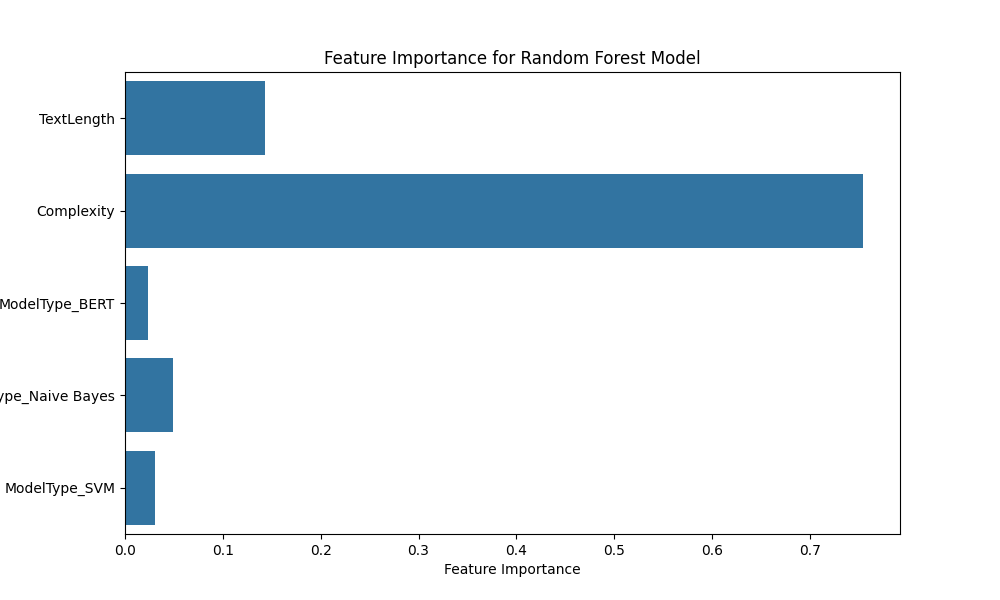
\includegraphics[width=0.9\columnwidth]{feature_importance_rf.png}
    \caption{Hva påvirker AI-ytelsen mest?}
\end{figure}

\begin{tcolorbox}[colback=purple!5!white, colframe=purple!75!black, title=Hvorfor Er Dette Viktig?]
Hvis vi kan gjøre AI bedre til å forstå tekster, kan vi få bedre kundeservice, automatiske sammendrag, og hjelp til studier. Det er viktig å fokusere på gode data og mye data for å få dette til.
\end{tcolorbox}

\section*{Oppsummering}
\begin{tcolorbox}[colback=gray!5!white, colframe=gray!75!black, title=Hva Fant Vi Ut?]
\begin{itemize}
    \item \textbf{Større datasett} gir bedre resultater.
    \item \textbf{Enklere tekster} gjør modellen mer nøyaktig.
    \item \textbf{Valg av modell} hjelper litt, men ikke like mye som datasettstørrelse og tekstvanskelighet.
\end{itemize}
\end{tcolorbox}

\end{multicols}

\end{document}
